\documentclass{article}

% if you need to pass options to natbib, use, e.g.:
%     \PassOptionsToPackage{numbers, compress}{natbib}
% before loading neurips_2026

\usepackage[final]{neurips_2026}

\usepackage[utf8]{inputenc} % allow utf-8 input
\usepackage[T1]{fontenc}    % use 8-bit T1 fonts
\usepackage{hyperref}       % hyperlinks
\usepackage{url}            % simple URL typesetting
\usepackage{booktabs}       % professional-quality tables
\usepackage{amsfonts}       % blackboard math symbols
\usepackage{nicefrac}       % compact symbols for 1/2, etc.
\usepackage{microtype}      % microtypography
\usepackage{xcolor}         % colors
\usepackage{graphicx}       % figures

\title{Beyond IID and Closed-Set Learning: Inductive Biases, Domain Shift, and Open-Set Recognition}

\author{%
  Zarman Ali Awan \\
  28100092 \\
  \texttt{zarman.awan@lums.edu.pk}
}

\begin{document}

\maketitle

\begin{abstract}
  One-paragraph summary: what you studied across the four tasks, the main
  findings, and a link to your code.
  GitHub repository: \url{https://github.com/alizarman786-prog/atml-assignment-1}
\end{abstract}

\section{Introduction}
Motivate the IID / closed-set breakdown; state the four tasks and the
research questions you will answer; preview the cross-task synthesis
question (what should a robust representation preserve, become invariant
to, and reject).

\section{Experimental Setup}
Shared conventions across tasks: seed 6304, datasets used (STL-10/Pets,
PACS, CIFAR-10/100), backbones, and any protocol details worth stating once
instead of repeating per task.

\section{Task 1: Inductive Biases and Feature Representations}
\label{sec:task1}

\subsection{Setup and Design Choices}
Dataset choice, cue-conflict class pairs and style strength, additional
color intervention, representation-visualization settings -- each stated
with a hypothesis and metric before interpreting results.

\subsection{Results}
\paragraph{Clean baseline.} Top-1 accuracy, macro-F1, mean max confidence
for the three heads and zero-shot CLIP (Table~\ref{tab:t1-clean}).

\begin{table}[h]
  \caption{Task 1 clean baseline. Fill in from \texttt{results/clean\_baseline\_seed6304.json}.}
  \label{tab:t1-clean}
  \centering
  \begin{tabular}{lccc}
    \toprule
    Model & Top-1 Acc. & Macro-F1 & Mean Max Conf. \\
    \midrule
    ResNet-50 (head)   & & & \\
    ViT-B/16 (head)    & & & \\
    CLIP ViT-B-32 (head) & & & \\
    CLIP zero-shot     & & & \\
    \bottomrule
  \end{tabular}
\end{table}

\paragraph{Color bias.} Grayscale and the chosen additional color
intervention: accuracy change and prediction consistency relative to clean.

\paragraph{Shape vs. texture.} Shape bias and coverage per model (report
$N_\text{shape}$, $N_\text{texture}$, $N_\text{other}$ counts too).

\paragraph{Translation.} Accuracy/consistency curve against displacement
(Figure~\ref{fig:translation}).

\begin{figure}[h]
  \centering
  % 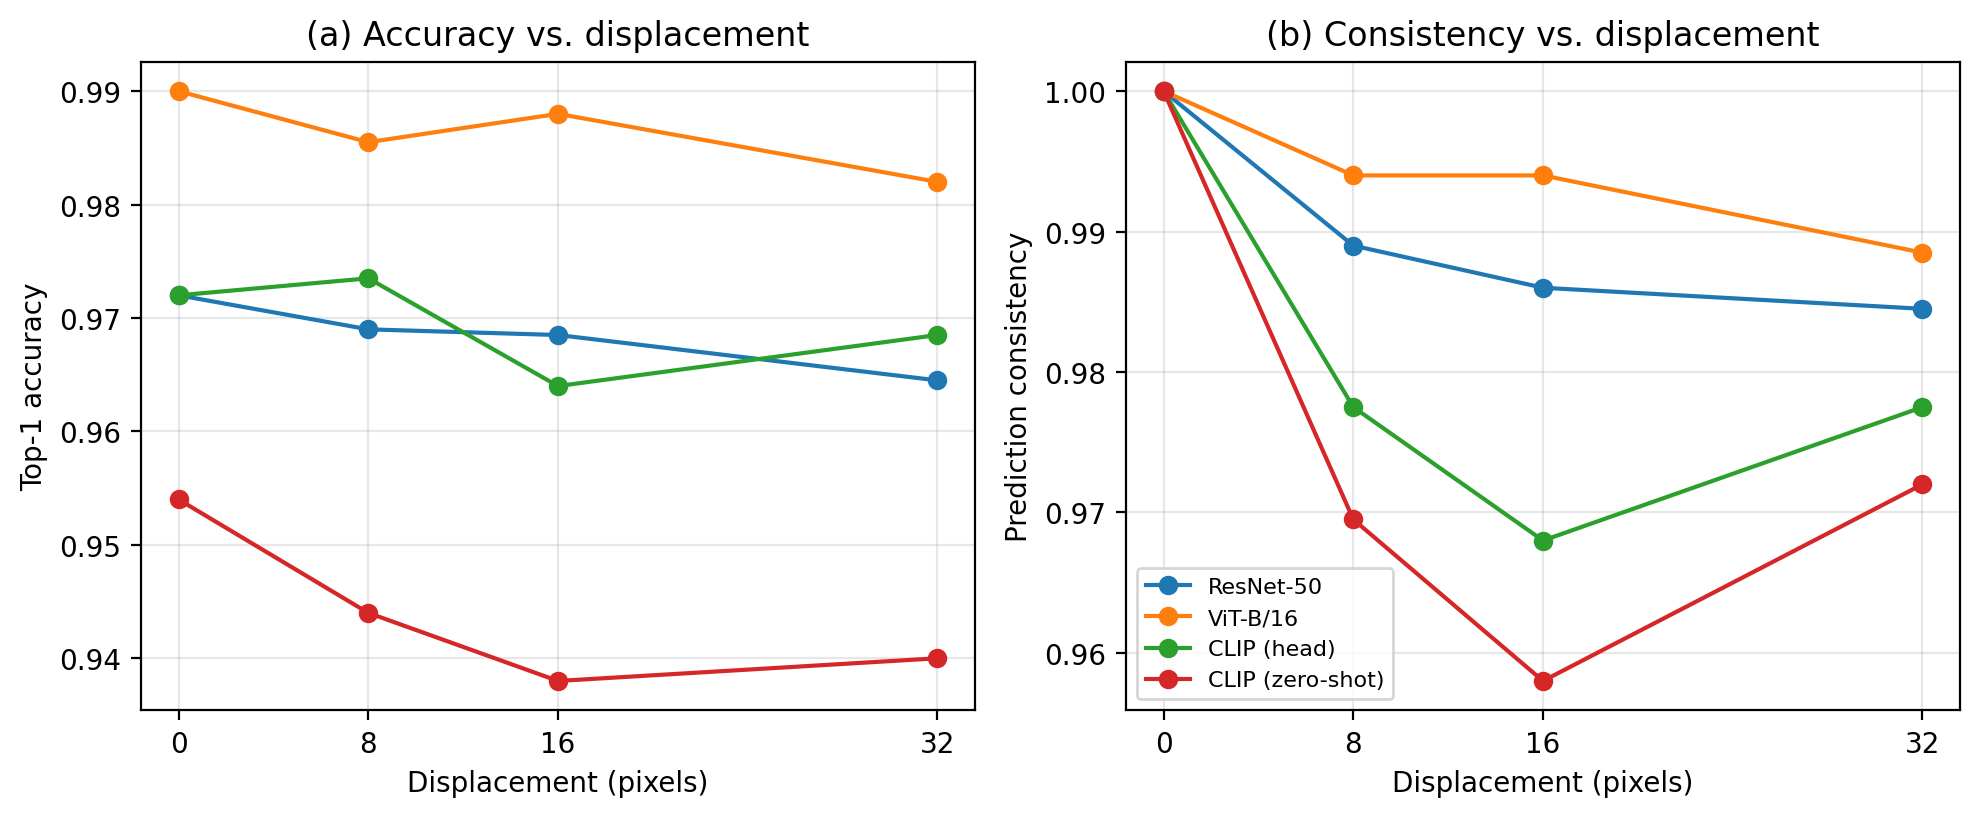
\includegraphics[width=0.7\linewidth]{figures/translation_curve.pdf}
  \caption{Accuracy and prediction consistency vs.\ translation displacement, per backbone.}
  \label{fig:translation}
\end{figure}

\paragraph{Patch structure.} Accuracy drop and prediction consistency under
4x4 patch shuffling.

\paragraph{Representation analysis.} Cosine stability $I_T$ per
intervention; t-SNE/UMAP visualizations of clean vs.\ transformed features.

\subsection{Discussion}
Answer Task 1's four research questions (cue reliance and coverage;
locality/positional sensitivity; prediction-representation agreement;
architecture vs.\ pretraining/data attribution).

\section{Task 2: Unsupervised Domain Adaptation}
\label{sec:task2}

\subsection{Setup}
PACS, Sketch as target, Photo/Art/Cartoon as sources; frozen BatchNorm
policy; training/optimization settings.

\subsection{Results}
Source-only, DAN, DANN, CDAN comparison table (per-source validation, mean,
target accuracy/macro-F1, target change, domain separability); alignment
training curves; per-class transfer; controlled $\lambda_\text{MMD}$ or
gradient-reversal-strength study.

\subsection{Discussion}
Answer Task 2's four research questions (domain gap and failing classes;
separability vs.\ recognition; class-conditional vs.\ marginal alignment;
alignment-strength trade-off).

\section{Task 3: Domain Generalization}
\label{sec:task3}

\subsection{Setup}
Same PACS protocol as Task 2, Sketch fully unseen; ERM/DAN-DG/SAM.

\subsection{Results}
ERM, DAN-DG, SAM comparison (mean-source, worst-source, Sketch
accuracy/macro-F1, change vs.\ ERM); source-domain separability; sharpness
proxy $\Delta_\text{sharp}$; per-class Sketch changes; controlled
$\lambda_\text{DG}$ or $\rho$ study.

\subsection{Discussion}
Answer Task 3's four research questions (mean/worst-source predicting
Sketch; DAN-DG invariance vs.\ class information; SAM sharpness vs.\
performance ranking; value of unlabeled target access, Task 2 vs.\ Task 3).

\section{Task 4: Open-Set Recognition}
\label{sec:task4}

\subsection{Setup}
CIFAR-10 known classes, CIFAR-100 near/far unknowns; Vanilla, GCSC, PROSER
(optionally RPL).

\subsection{Results}
MSP/MLS/Energy/Mahalanobis comparison on the vanilla model (near/far/all
AUROC, calibrated rejection); Vanilla vs.\ GCSC vs.\ PROSER with MLS
(+ PROSER placeholder score); score-distribution/ROC figure; failure cases.

\subsection{Discussion}
Answer Task 4's four research questions (semantic similarity and rejection;
what each score captures; GCSC's effect on CSA vs.\ OSR; PROSER's
placeholder trade-off).

\section{Cross-Task Discussion}
Visual cues and distribution shift; invariance vs.\ discriminability; the
importance of target-domain access; recognition vs.\ rejection; overall
synthesis of what a robust representation should preserve, suppress, and
reject.

\section{Conclusion}
Summarize the cross-task synthesis argument.

\begin{ack}
Optional: acknowledge any TA/instructor help, compute resources, etc. (Not
required for a course assignment; remove this section if you have nothing
to declare.)
\end{ack}

\section*{References}
Use \verb+\citet+/\verb+\citep+ with a \texttt{.bib} file (natbib is loaded
by default) rather than hand-formatting references. References do not
count toward the 8-page limit. At minimum, cite: Geirhos et al. (2019),
Ganin et al. (2016), Long et al. (2018), Foret et al. (2021), Vaze et al.
(2022), Zhou et al. (2021), plus any optional readings you used.

\appendix
\section{Appendix (optional)}
Implementation details or extra results only -- not required reading for
graders and cannot substitute for required evidence in the main text.

\end{document}
